%%%%%%%%%%%%%%%%%%%%%%%%%%%%%%%%%%%%%%%%%%%%%%%%
% 1. Document Class
%%%%%%%%%%%%%%%%%%%%%%%%%%%%%%%%%%%%%%%%%%%%%%%%
 
 % The first command you will always have will declare your document class. This tells LaTeX what type of document you are creating (article, presentation, poster, etc). 
% \documentclass is the command
% in {} you specify the type of document
% in [] you define additional parameters
 
\documentclass[a4paper,12pt]{article} % This defines the style of your paper

% We usually use the article type. The additional parameters are the format of the paper you want to print it on and the standard font size. For us this is a4paper and 12pt.

%%%%%%%%%%%%%%%%%%%%%%%%%%%%%%%%%%%%%%%%%%%%%%%%
% 2. Packages
%%%%%%%%%%%%%%%%%%%%%%%%%%%%%%%%%%%%%%%%%%%%%%%%

% Packages are libraries of commands that LaTeX can call when compiling the document. With the specialized commands you can customize the formatting of your document.
% If the packages we call are not installed yet, TeXworks will ask you to install the necessary packages while compiling.

% First, we usually want to set the margins of our document. For this we use the package geometry. We call the package with the \usepackage command. The package goes in the {}, the parameters again go into the [].
\usepackage[top = 2.5cm, bottom = 2.5cm, left = 2.5cm, right = 2.5cm]{geometry} 

% Unfortunately, LaTeX has a hard time interpreting German Umlaute. The following two lines and packages should help. If it doesn't work for you please let me know.
\usepackage[T1]{fontenc}
\usepackage[utf8]{inputenc}
\usepackage{amsmath}
\usepackage{cancel}
\usepackage{amssymb}
\usepackage{pgfplots}
\usepackage{amsmath}
\usepackage{siunitx}

\usepackage{physics}
\usepackage{tikz}
\usepackage[outline]{contour} % glow around text
\usetikzlibrary{patterns,snakes}
\usetikzlibrary{arrows.meta} % for arrow size
\contourlength{0.4pt}

\contourlength{1.0pt}
\usetikzlibrary{angles,quotes} % for pic (angle labels)
\usetikzlibrary{arrows.meta}
\usetikzlibrary{decorations.markings}
%\usetikzlibrary{bending} % for arrow head angle
\tikzset{>=latex} % for LaTeX arrow head
\usepackage{xcolor}

\colorlet{xcol}{blue!60!black}
\colorlet{myred}{red!80!black}
\colorlet{myblue}{blue!80!black}
\colorlet{mygreen}{green!40!black}
\colorlet{myorange}{orange!90!black}
\colorlet{mypurple}{red!50!blue!90!black!80}
\colorlet{mydarkred}{myred!80!black}
\colorlet{mydarkblue}{myblue!80!black}
\tikzstyle{xline}=[xcol,thick]
\tikzstyle{width}=[{Latex[length=5,width=3]}-{Latex[length=5,width=3]},thick]
\tikzset{
  traj/.style 2 args={xline,postaction={decorate},decoration={markings,
    mark=at position #1 with {\arrow{<}},
    mark=at position #2 with {\arrow{<}}}
  }
}
\def\tick#1#2{\draw[thick] (#1)++(#2:0.12) --++ (#2-180:0.24)}
\def\N{100} % number of samples


\colorlet{xcol}{blue!70!black}
\colorlet{darkblue}{blue!40!black}
\colorlet{myred}{red!65!black}
\tikzstyle{mydashed}=[xcol,dashed,line width=0.25,dash pattern=on 2.2pt off 2.2pt]
\tikzstyle{axis}=[->,thick] %line width=0.6
\tikzstyle{ell}=[{Latex[length=3.3,width=2.2]}-{Latex[length=3.3,width=2.2]},line width=0.3]
\tikzstyle{dx}=[-{Latex[length=3.3,width=2.2]},darkblue,line width=0.3]
\tikzstyle{ground}=[preaction={fill,top color=black!10,bottom color=black!5,shading angle=20},
                    fill,pattern=north east lines,draw=none,minimum width=0.3,minimum height=0.6]
\tikzstyle{mass}=[line width=0.6,blue!30!black,fill=blue!40!black!10,rounded corners=1,
                  top color=blue!40!black!20,bottom color=blue!40!black!10,shading angle=20]
\tikzstyle{spring}=[line width=0.8,blue!7!black!80,snake=coil,segment amplitude=5,segment length=5,line cap=round]
\tikzset{>=latex} % for LaTeX arrow head
\tikzstyle{force}=[->,myred,very thick,line cap=round]
\def\tick#1#2{\draw[thick] (#1)++(#2:0.1) --++ (#2-180:0.2)}

% The following two packages - multirow and booktabs - are needed to create nice looking tables.
\usepackage{multirow} % Multirow is for tables with multiple rows within one cell.
\usepackage{booktabs} % For even nicer tables.

% As we usually want to include some plots (.pdf files) we need a package for that.
\usepackage{graphicx} 

% The default setting of LaTeX is to indent new paragraphs. This is useful for articles. But not really nice for homework problem sets. The following command sets the indent to 0.
\usepackage{setspace}
\setlength{\parindent}{0in}

% Package to place figures where you want them.
\usepackage{float}

% The fancyhdr package let's us create nice headers.
\usepackage{fancyhdr}

% Citing references will be hyperlinked and blue
\usepackage[colorlinks=true,linkcolor=blue]{hyperref}

\usepackage{tikz}
\usetikzlibrary{tikzmark}

%%%%%%%%%%%%%%%%%%%%%%%%%%%%%%%%%%%%%%%%%%%%%%%%
% 3. Header (and Footer)
%%%%%%%%%%%%%%%%%%%%%%%%%%%%%%%%%%%%%%%%%%%%%%%%

% To make our document nice we want a header and number the pages in the footer.

\pagestyle{fancy} % With this command we can customize the header style.

\fancyhf{} % This makes sure we do not have other information in our header or footer.

\lhead{\footnotesize }% \lhead puts text in the top left corner. \footnotesize sets our font to a smaller size.

%\rhead works just like \lhead (you can also use \chead)
\rhead{\footnotesize Collins \thepage} %<---- Fill in your lastnames.

% Similar commands work for the footer (\lfoot, \cfoot and \rfoot).
% We want to put our page number in the center.
\cfoot{\footnotesize} 


%%%%%%%%%%%%%%%%%%%%%%%%%%%%%%%%%%%%%%%%%%%%%%%%
% 4. Your document
%%%%%%%%%%%%%%%%%%%%%%%%%%%%%%%%%%%%%%%%%%%%%%%%

% Now, you need to tell LaTeX where your document starts. We do this with the \begin{document} command.
% Like brackets every \begin{} command needs a corresponding \end{} command. We come back to this later.

\begin{document}


%%%%%%%%%%%%%%%%%%%%%%%%%%%%%%%%%%%%%%%%%%%%%%%%
%%%%%%%%%%%%%%%%%%%%%%%%%%%%%%%%%%%%%%%%%%%%%%%%

%%%%%%%%%%%%%%%%%%%%%%%%%%%%%%%%%%%%%%%%%%%%%%%%
% Title section of the document
%%%%%%%%%%%%%%%%%%%%%%%%%%%%%%%%%%%%%%%%%%%%%%%%

% For the title section we want to reproduce the title section of the Problem Set and add your names.

\thispagestyle{empty} % This command disables the header on the first page. 

\begin{tabular}{p{15.5cm}} % This is a simple tabular environment to align your text nicely 
\\ Collin Collins \\
MATH 3400\\
SI Session 8 Exam 2 Review\\
12 March 2024 \\
\hline % \hline produces horizontal lines.

\end{tabular} 

\subsection*{Problem 1}
Find $y(\frac{3}{10})$ using Euler's Method
$$ y' = 2x + 3y \quad;\quad y(0) = 1 \quad;\quad h=\frac{1}{10} $$

Try it out before looking at the solution.

\pagebreak

\subsection*{Solution to Problem 1:}

Euler's method is a numerical method for solving differential equations. In this case, we are given an initial condition, a step size, and we are asked to find the value of $y(\frac{3}{10})$. To do this using Euler's Method, we should remember the formula:
$$ y_{n+1} = y_n + hf(x_n, y_n). $$
Since $f(x_n, y_n)$ is our slope field, we could write it in a nicer way as:
$$ \boxed{y_{n+1} = y_n + hy'_n} $$

I think that this way is a lot easier to remember because we can read this equation in a nice way.\\

 It says "The next approximation of $y$ is the current approximation of $y$ plus a contribution from the slope (derivative) at the current point, scaled by the step size $h$."\\
 
 Now, let's start off by thinking about what our initial condition means:
 
 $$ y(0)=1\quad \text{ means }\quad \begin{matrix}x_0 = 0 \\ y_0 = 1 \end{matrix}$$
 $h$ is the step size in the $x$-direction. So, already we have the following information:
 
$$ 
\left(\begin{matrix}
 	\text{iteration} & x_n & y_n \\
 	0 & 0 & 1 \\
 	1 & 1/10 & y_1 \\
 	2 & 2/10 & y_2 \\
 	3 & 3/10 & y_3
\end{matrix}\right)
 $$
 In order to find $y_3$, we need to find $y_2$. To find $y_2$, we need to know $y_1$. So let's begin.
 
 $$ y_{0+1} = y_0 + h\underbrace{y'_0}_{\text{find this}}. $$
 $$ y_0' = 2x_0 + 3y_0 \quad\implies\quad y_0' = 2(0) + 3(1) \quad\implies\quad y_0' = 3. $$
 $$ y_1 = 1 + \frac{1}{10}(3) \quad\implies\quad y_1 = \frac{10}{10} + \frac{3}{10} \quad\implies\quad \boxed{y_1 = \frac{13}{10}} $$
 $$ 
\left(\begin{matrix}
 	\text{iteration} & x_n & y_n \\
 	0 & 0 & 1 \\
 	1 & 1/10 & 13/10 \\
 	2 & 2/10 & y_2 \\
 	3 & 3/10 & y_3
\end{matrix}\right)
 $$
 Now, we use $y_1$ to find $y_2$. By the way, we wont be able to use a calculator on the exam, so working with fractions will help immensely.
 $$ y_{1+1} = y_1 + h\underbrace{y_1'}_{\text{find this}}. $$
 $$ y_1' = 2x_1 + 3y_1 \quad\implies\quad y_1' = 2\left(\frac{1}{10}\right) + 3\left(\frac{13}{10}\right) \quad\implies\quad y'_1 = \frac{2}{10} + \frac{39}{10} \quad\implies\quad y_1' = \frac{41}{10}.  $$
 $$ y_2 = \frac{13}{10} + \frac{1}{10}\left(\frac{41}{10}\right) \quad\implies\quad y_2 = \frac{13}{10} + \frac{41}{100} \quad\implies\quad y_2 = \frac{130}{100} + \frac{41}{100} \quad\implies\quad \boxed{y_2 = \frac{171}{100}} $$
  $$ 
\left(\begin{matrix}
 	\text{iteration} & x_n & y_n \\
 	0 & 0 & 1 \\
 	1 & 1/10 & 13/10 \\
 	2 & 2/10 & 171/100 \\
 	3 & 3/10 & y_3
\end{matrix}\right)
 $$
 Finally, we use $y_2$ to find $y_3$.
 $$ y_{2 + 1} = y_2 + h\underbrace{y_2'}_{\text{find this}} $$
 $$ y'_2 = 2x_2 + 3y_2 \quad\implies\quad y_2' = 2\left(\frac{2}{10}\right) + 3\left(\frac{171}{100}\right) \quad\implies\quad y_2' = \frac{40}{100} + \frac{513}{100} \quad\implies\quad \boxed{y_2' = \frac{553}{100}} $$
 $$ y_3 = \frac{171}{100} + \frac{1}{10}\left(\frac{553}{100}\right) \quad\implies\quad y_3 = \frac{1710}{1000} + \frac{553}{1000} \quad\implies\quad \underline{\boxed{y_3 = \frac{2263}{1000}}} $$
  $$ 
\left(\begin{matrix}
 	\text{iteration} & x_n & y_n \\
 	0 & 0 & 1 \\
 	1 & 1/10 & 13/10 \\
 	2 & 2/10 & 171/100 \\
 	3 & 3/10 & 2263/1000
\end{matrix}\right)
 $$
\pagebreak

\subsection*{Problem 2}
A thermometer is taken from a room where the temperature is $20^{\circ}\mathrm{C}$ to the outdoors, where the temperature is $5^{\circ} \mathrm{C}$. After one minute the thermometer reads $12^{\circ} \mathrm{C}$.\\

(a) What will the temperature be after one more minute of cooling?\\
(b) Sketch the equation that describes the temperature as a function of time.\\

Try it out before looking at the solution.

\pagebreak

\subsection*{Solution to Problem 2:}
\textbf{(a)}\\
Newton's Law of Cooling is given as:
$$\frac{d T}{d t}=k\left(T-T_m\right)$$
From the problem, we know that; the ambient temperature $T_m$ is 5$^{\circ}$C; at $t=0$, the temperature is 20$^{\circ}$C; at $t=1$ min, the temperature is 12$^{\circ}$C.\\

Let's use this information to answer part (a):
$$ \frac{dT}{dt} = k(T-5). $$
This differential equation is separable:
$$ \frac{1}{T-5}dT = k dt \quad\implies\quad \ln{|T-5|} = kt + C \quad\implies\quad T-5 = Ae^{kt} \quad\implies\ldots$$
$$ \ldots\implies\quad T_g(t) = Ae^{kt} + 5. $$
We have that $T(0)=20$, so let's determine the value of $A$.
$$ T(0)=20\quad:\quad 20 = Ae^{0}+5 \quad\implies\quad A = 15. $$
We now have:
$$ T_g(t) = 15e^{kt} + 5. $$
It is still general because we have a free parameter, $k$. To determine its value, let's use another condition---that $T(1)=12$.
$$ T(1)=12\quad:\quad 12 = 15e^{k(1)} + 5 \quad\implies\quad e^k=\frac{12-5}{15} \quad\implies\quad k=\ln{\left(\frac{7}{15}\right)}.$$
With the cooling rate, we can determine the temperature after another minute, $T(2)$.
$$ T(2) = 15e^{\ln{\left(\frac{7}{15}\right)}(2)} + 5 \quad\implies\quad T(2) = 15e^{\ln{\left(\frac{49}{225}\right)}} + 5  \quad\implies\quad T(2) = 15\left(\frac{49}{225}\right) + 5 \quad\ldots$$
$$ \ldots\implies\quad T(2) = \frac{49}{15} + 5 \quad\implies\quad T(2) = \frac{49 +75}{15} \quad\implies\quad \underline{\boxed{T(2) = \frac{124}{15}}} $$

\pagebreak

\textbf{(b)}\\
We are plotting

$$ T(t) =  15e^{\ln{\left(\frac{7}{15}\right)}t} + 5 $$

\begin{center}
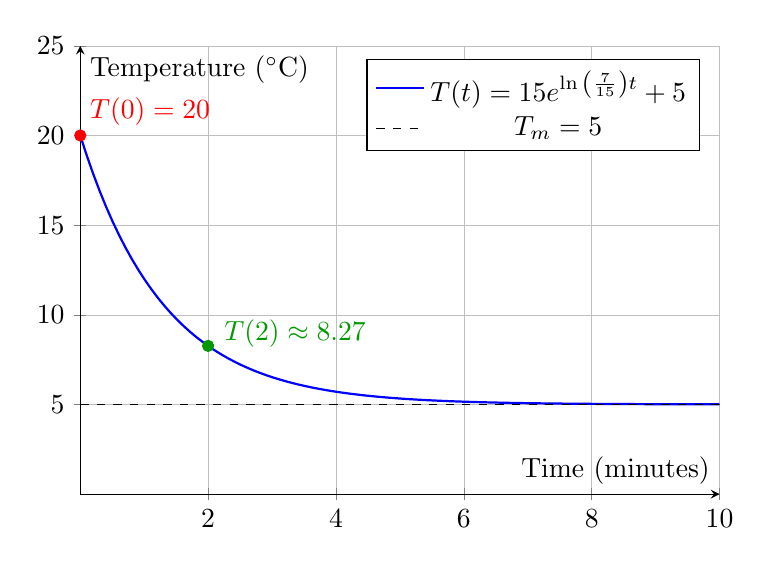
\begin{tikzpicture}[scale=1]
\begin{axis}[
width=0.8\textwidth,
height=0.6\textwidth,
xlabel={Time (minutes)},
ylabel={Temperature (\si{\degree}C)},
xmin=0, xmax=10,
ymin=0, ymax=25,
grid=both,
grid style={line width=.1pt, draw=gray!40},
major grid style={line width=.2pt,draw=gray!50},
axis lines=middle,
samples=100,
domain=0:10,
legend pos=north east,
legend cell align={center},
]

\addplot[blue, thick] {15*exp(ln(7/15)*x) + 5};
\addlegendentry{$T(t) = 15e^{\ln{\left(\frac{7}{15}\right)}t} + 5$}

\addplot[dashed, black] coordinates {(0, 5) (10, 5)};
\addlegendentry{$T_m = 5$}

\addplot[only marks, red, mark=*, mark size=2pt] coordinates {(0, 20)};
\node[above right, red] at (axis cs:0, 20) {$T(0) = 20$};

\addplot[only marks, green!60!black, mark=*, mark size=2pt] coordinates {(2.0, 8.266666667)};
\node[below right, green!60!black] at (axis cs:2.1, 10.266666667) {$T(2) \approx 8.27$};

\end{axis}
\end{tikzpicture}
\end{center}

\pagebreak

\subsection*{Problem 3}
Consider a mass-spring system, described by the equation $mx'' + cx' + kx = 0$.\\

Imagine you're determining the damping effect on a 1 kg mass moving across a surface. Using a spring with a stiffness coefficient of $k = 1000$ N/m, you connect it to the mass and secure the other end to a stationary object. By stretching the spring and releasing it, you observe the mass undergoes oscillations at a frequency of 2 Hz, indicating the system is underdamped.\\

Determine the value of the damping coefficient $c$.\\

\begin{center}
% HORIZONTAL spring - axis, rest position
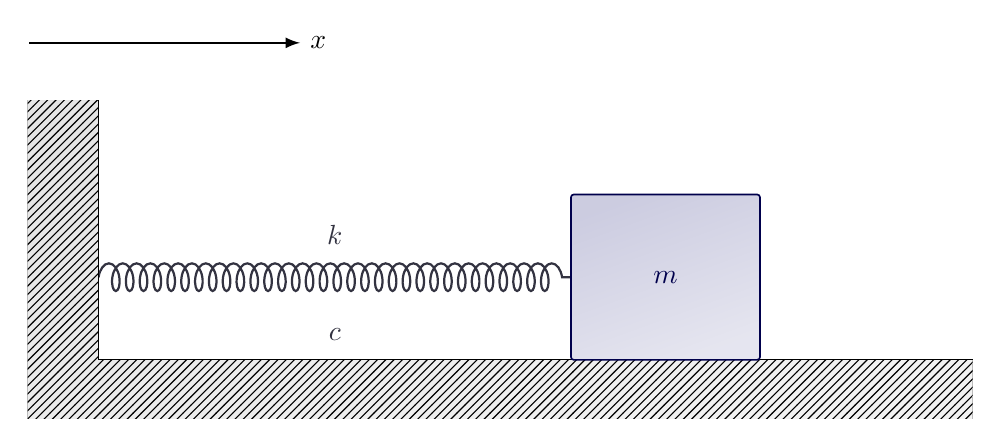
\begin{tikzpicture}[scale=3]
  \def\H{1.1}  % wall height
  \def\T{0.3}  % wall thickness
  \def\W{3.7}  % ground length
  \def\D{0.25} % ground depth
  \def\h{0.7}  % mass height
  \def\w{0.8}  % mass width
  \def\x{2.0}  % mass x position
  \def\y{1.22*\H} % x axis y position
 
  % AXIS
  \draw[axis] (\x-0.62*\W,\y) -- (\x-0.31*\W,\y) node[right] {$x$};
  
  % SPRING & MASS
  \draw[spring] (0,\h/2) --++ (\x,0) node[midway,above=8pt] {$k$} node[midway,below=15pt] {$c$};
  \draw[ground] (0,0) |-++ (-\T,\H) |-++ (\T+\W,-\H-\D) -- (\W,0) -- cycle;
  \draw (0,\H) -- (0,0) -- (\W,0);
  \draw[mass] (\x,0) rectangle++ (\w,\h) node[midway] {$m$};
  
\end{tikzpicture}
\end{center}

Try it out before looking at the solution.

\pagebreak

\subsection*{Solution to Problem 3:}
Let's start off by working symbolically with our system:
$$ mx'' + cx' + kx = 0 $$
If $m$, $c$, and $k$ are all constants, then this is a second-order, linear, constant coefficient, homogenous differential equation. This immediately motivates us to find the discriminant to determine the form of the general solution:
$$ D = b_o^2 - 4a_oc_o \quad\text{ where $a_o$, $b_o$, and $c_o$ are $m$, $c$, and $k$, respectively.} $$
$$ D = c^2 - 4mk $$
Now, let's think about this. We know what $m$ and $k$ are, but we are trying to determine the value of $c$. We should revisit our problem and look for more information.\\

The problem states that the system is underdamped. Since this is a physical system, there is some physical interpretation that we can assign to each case of the discriminant trichotomy.\\

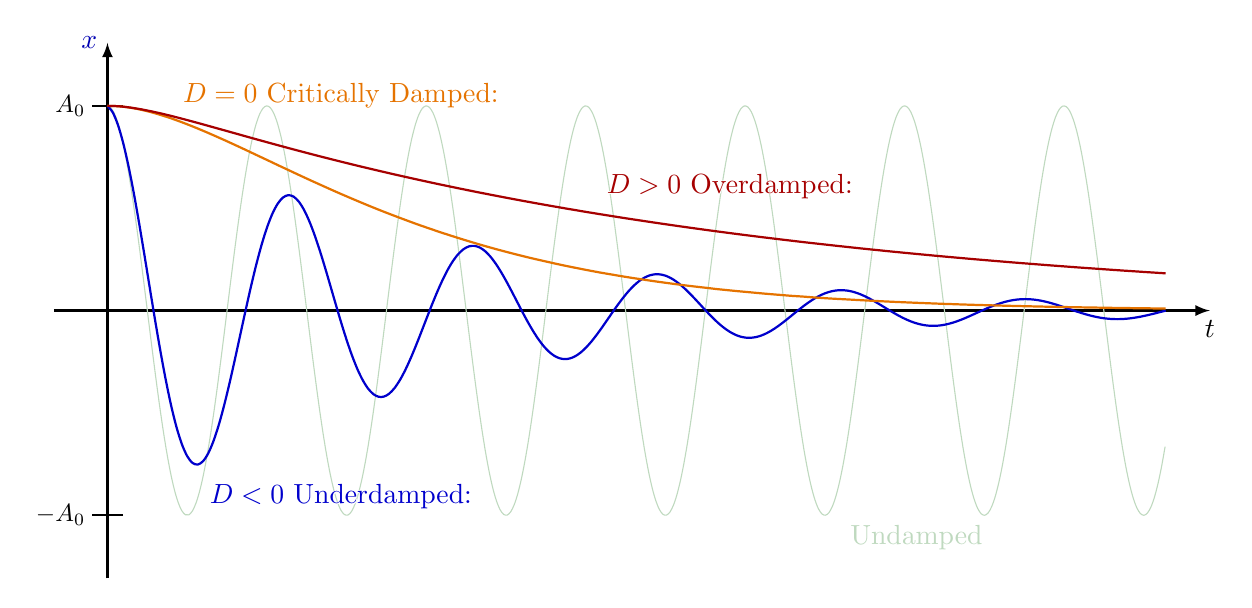
\begin{tikzpicture}[scale=2]
  \def\xmax{7.0} % max x axis
  \def\ymax{1.7} % max y axis
  \def\A{1.3}
  \def\om{(6.5/(0.94*\xmax))} % natural omega_0
  \def\Za{0.50} % zeta underdamped 1
  \def\Zb{0.95} % zeta underdamped 2
  \def\Zc{1.00} % zeta critically damped
  \def\Zd{2.00} % zeta overdamped
  \def\Ga{(\Za*\om)} % gamma underdamped 1
  \def\Gb{(\Zb*\om)} % gamma underdamped 2
  \def\Gc{\om}       % gamma critically damped
  \def\Gd{(\Zd*\om)} % gamma overdamped
  \def\Wa{(\om*sqrt(1-\Za*\Za)}  % omega underdamped 1
  \def\Wb{(\om*sqrt(1-\Zb*\Zb)}  % omega underdamped 2
  \def\Wd{(\om*sqrt(\Zd*\Zd-1))} % omega overdamped
  
  % AXIS
  \draw[->,thick] (0,-\ymax) -- (0,\ymax) node[left,xcol] {$x$};
  \draw[->,thick] (-0.2*\ymax,0) -- (\xmax,0) node[below] {$t$};
  \tick{0,\A}{0} node[left=-1,scale=0.9] {$A_0$};
  \tick{0,-\A}{0} node[left=-1,scale=0.9] {$-A_0$};
  
  % PLOT
  \draw[xline,mygreen!25,thin,samples=200+\N,smooth,variable=\t,domain=0:0.96*\xmax]
    plot(\t,{\A*cos(360*\om*\t)});
  \draw[xline,myblue,samples=100+\N,smooth,variable=\t,domain=0:0.96*\xmax]
    plot(\t,{\A*exp(-\Ga*\t)*cos(360*\Wa*\t)});
      \draw[xline,myorange,samples=\N,smooth,variable=\t,domain=0:0.96*\xmax]
    plot(\t,{\A*(1+\Gc*\t)*exp(-\Gc*\t)});
  \draw[xline,myred,samples=\N,smooth,variable=\t,domain=0:0.96*\xmax]
    plot(\t,{\A/2*( (1+\Gd/\Wd)*exp((\Wd-\Gd)*\t) + (1-\Gd/\Wd)*exp(-(\Wd+\Gd)*\t))});
  %\node[above=4] at (0.15*\xmax,{\A*exp(-0.15*\xmax/\T)}) {$e^{-\frac{b}{2m}t}$};
   
  % NODES
  \node[below,mygreen!25] at ({5.20*\om},-1.00*\A) {$\text{Undamped}$};
  \node[below,myblue]   at ({1.5*\om},-0.8*\A) {\contour{white}{$D<0\text{ Underdamped:}$}};
  \node[above,myorange]   at ({1.5*\om}, 0.94*\A) {$D=0\text{ Critically Damped:}$};
  \node[above,myred]      at ({4*\om}, 0.50*\A) {\contour{white}{$D>0\text{ Overdamped:}$}};
  
\end{tikzpicture}


The problem tells us that the mass oscillates with some frequency, $f=2$ Hz. Based on the figure above, the only case where there is any oscillation occurs for $D<0$.\\

So, just by thinking about it, we have arrived at the conclusion that our solution will have the following form:
$$ x_g(t) =e^{-(Re) t}\bigg[C_1\cos [(Im) t]+C_2\sin [(Im) t]\bigg]. $$
and that:
$$ D<0. $$
Here, the frequency at which the mass oscillates is whatever is in the argument of the sine and cosine. We should be careful to note that this frequency is an angular frequency. To convert what we were given into an angular frequency:
$$ (Im) =  \omega_{\text{damped}} = 2\pi f. $$
Knowing this, we will use the quadratic formula to find the damping coefficient, $c$.
$$ \lambda_{1,2} = \frac{-b_o \pm \sqrt{D}}{2a_o} \quad\implies\quad \lambda_{1,2} = -\frac{c}{2m} \pm \frac{\sqrt{D}}{2m} \quad \implies\ldots$$
$$\ldots\implies\quad \lambda_{1,2} = -\frac{c}{2m} \pm \frac{\sqrt{c^2-4mk}}{2m} \quad\implies\quad \lambda_{1,2} = -\frac{c}{2m} \pm \sqrt{\frac{c^2-4mk}{4m^2}} = (Re)\pm (Im)i  $$
Here, $\sqrt{\frac{c^2-4mk}{4m^2}}$ must equal $(Im)i$:
$$ \sqrt{\frac{c^2-4mk}{4m^2}} = (Im)i.$$
This is one equation with one unknown, let's use the fact that $(Im)=2\pi f$ to solve for $c$:
$$ \sqrt{\frac{c^2-4mk}{4m^2}} = 2\pi fi \quad\implies\quad c^2 -4mk = 4m^2(2\pi f i)^2 \quad\implies\ldots $$
$$\ldots\implies\quad  c^2 = -16\pi^2 m^2f^2 + 4mk \quad\implies\quad c = \sqrt{4(mk-4\pi^2m^2f^2)}\quad\implies\ldots$$
$$ \ldots\implies\quad c = 2\sqrt{m(k-4\pi^2mf^2)}. $$
From here, we can plug in our numbers, being careful with our units:
$$ c = 2\sqrt{1(1000-4\pi^2(1)(2^2))} \quad\implies\quad \boxed{c= 2\sqrt{1000-16\pi^2}} $$
Let's do some quick dimensional analysis to find our out units:
$$c \overset{u}= [\text{ }]\sqrt{[\text{kg}]\left(\left[\frac{\text{N}}{\text{m}}\right] - [\text{ }][\text{ }]^2[\text{kg}]\left[\frac{1}{\text{s}}\right]^2\right)} \quad\implies\quad c\overset{u}= \sqrt{\left[\frac{[\text{kg}][\text{kg}][\text{m}]}{[\text{m}][\text{s}]^2} - \frac{[\text{kg}]^2}{[\text{s}]^2}\right]} \quad\implies\ldots $$
$$ c\overset{u}=\sqrt{\frac{[\text{kg}]^2}{[\text{s}]^2}} \quad\implies\quad \boxed{c\overset{u}=\left[\frac{\text{kg}}{\text{s}}\right]} $$
Finally,
$$ \underline{\boxed{c= 2\sqrt{1000-16\pi^2} \text{ }\left[\frac{\text{kg}}{\text{s}}\right]}}  $$




If you wanted to do this in less that five minutes at the expense of having to memorize more things, you could've used the relation that:
$$ c=2m\sqrt{\omega^2_{\text{natural}} - \omega^2_{\text{damped}}}, $$
which can be derived from the following step used above:
$$c = \sqrt{4(mk-4\pi^2m^2f^2)} \quad\implies\quad c = 2\sqrt{m^2\left(\frac{k}{m}-2^2\pi^2f^2\right)}\quad\implies\ldots $$
$$\ldots\implies\quad \boxed{c = 2m\sqrt{\omega_{\text{natural}}^2 - \omega_{\text{damped}}^2}  } $$

\pagebreak

\subsection*{Problem 4}

Use the Reduction of Order technique to find $y_2(x)$:

$$ y^{\prime \prime}+9 y=0 \quad;\quad y_1=\sin{(3x)} $$\

Try it out before looking at the solution.

\pagebreak

\subsection*{Solution to Problem 4:}

Since this is a second-order, constant-coefficient, homogenous, linear differential equation, the full general solution will be:

$$ y_g = C_1y_1 + C_2y_2. $$

We are given that $y_1 = \sin{(3x)}$, so let's use the reduction of order formula to find $y_2$:

$$ y_2=y_1 \int \frac{e^{-\int p d x}}{y_1^2} d x. $$


Substituting what is known:

$$ y_2 = \sin{(3x)} \int \frac{e^{-\int (0)dx}}{\sin^2{(3x)}}dx \quad\implies\quad y_2 = \sin{(3x)} \int \frac{e^c}{\sin^2{(3x)}}dx \quad\implies\ldots $$
$$\ldots\implies\quad y_2 = C\sin{(3x)}\int \csc^{2}{(3x)} dx \quad\implies\quad y_2 = -\frac{C}{3}\sin{(3x)}\cot{(3x)} \quad\implies\ldots $$
$$ \ldots\implies\quad y_2 = A\sin{(3x)}\frac{\cos{(3x)}}{\sin{(3x)}} \quad\implies\quad y_2=A\cos{(3x)}. $$
Since our general solution already contains our constants, we can write $y_2$ as:
$$ \underline{\boxed{y_2 = \cos{(3x)}}} $$

\pagebreak

\subsection*{Problem 5}

Solve the following IVP using the method of Undetermined Coefficients.

$$ y'' + 6y' + 5y = 9e^{-5t} \quad:\quad y(0)=0\quad,\quad y'(0)=-\frac{9}{4}.
$$\

Try it out before looking at the solution.

\pagebreak

\subsection*{Solution to Problem 5:}
Let's start solving this problem by finding the complementary solution. To do this, we will find the determinant.
$$ D = b^2 -4ac \quad\implies\quad D = (6)^2 -4(1)(5) \quad\implies\quad D=16 \quad\therefore\quad D>0. $$
$$ y_c = C_1e^{-t} + C_2e^{-5t} \text{ where } \lambda_{1,2} = \frac{-b \pm \sqrt{D}}{2a}.$$
Finding the roots:
$$ \lambda_{1,2} = \frac{-6 \pm \sqrt{16}}{2(1)} \quad\implies\quad \lambda_1 = -1 \text{ and } \lambda_2 = -5. $$
$$ y_c = C_1e^{-t} + C_2e^{-5t}. $$
With our complementary solution, we can now start finding our particular solution. To use the method of Undetermined Coefficients, we will determine what a suitable guess is. Here, notice that at first we might consider $y_{p_g} = Ae^{-5t}$, but notice that this is linearly independent with the second half of our complementary solution. To ensure linear independence, let's add a factor of $t$.
$$ y_{p_g} = Ate^{-5t}. $$
Taking the derivatives:
$$ y_{p_g}' = Ae^{-5t} - 5Ate^{-5t}. $$
$$ y_{p_g}'' = -5Ae^{-5t} - 5Ae^{-5t} + 25Ate^{-5t}. $$
Let's plug these into the left-hand side of the original differential equation in order to determine the value of $A$ for which we have a true statement.
$$ \left[-10Ae^{-5t} + 25Ate^{-5t}\right] + 6\left[Ae^{-5t} - 5Ate^{-5t}\right] + 5\left[Ate^{-5t}\right] = 9e^{-5t}. $$
Now, let's group terms by their functions (not their coefficients).

$$\left[-10A\underline{e^{-5t}} + 25A\underline{\underline{te^{-5t}}}\right] + 6\left[A\underline{e^{-5t}} - 5A\underline{\underline{te^{-5t}}}\right] + 5\left[A\underline{\underline{te^{-5t}}}\right] = 9e^{-5t} \quad\implies\ldots$$
$$ \implies\ldots\quad [-10A + 6A]e^{-5t} + [25A -30A + 5A]te^{-5t} = [9]e^{-5t} + [0]te^{-5t}. $$
Now, we see that $-4A$ must equal 9 and $0A$ must equal 0.
$$ -4A=9 \quad\implies\quad A = -\frac{9}{4}.$$
Our particular solution is now:
$$ y_p = -\frac{9}{4}te^{-5t}. $$
Our full general solution is the combination of our particular and complementary solutions, so:
$$ \boxed{y_g(t) = C_1e^{-t} + C_2e^{-5t} -\frac{9}{4}te^{-5t}}  $$
Since we are given initial conditions, let's find our constants: $C_1$ and $C_2$:
$$ y(0)=0 \quad:\quad 0=C_1 + C_2 + 0 \quad\implies\quad \boxed{C_1 + C_2 = 0} $$
To use the initial condition for the derivative, let's take the derivative:
$$ y_g'(t) = -C_1e^{-t} -5C_2e^{-5t} -\frac{9}{4}e^{-5t} +\frac{45}{4}te^{-5t}. $$
$$ y'(0) = \frac{9}{4} \quad:\quad \frac{9}{4} = -C_1 -5C_2 - \frac{9}{4} \quad\implies\quad \boxed{C_1 + 5C_2 = 0} $$
Let's set up a matrix to find the values of $C_1$ and $C_2$:
$$
\left(\begin{matrix}
	1 & 1 & \vline & 0 \\
	1 & 5 & \vline & 0
\end{matrix}\right)
\quad\overset{-R_1 + R_2}\implies\quad
\left(\begin{matrix}
	1 & 1 & \vline & 0 \\
	0 & 4 & \vline & 0
\end{matrix}\right)
\quad\overset{-\frac{1}{4}R_2 + R_1}\implies\quad
\left(\begin{matrix}
	1 & 0 & \vline & 0 \\
	0 & 1 & \vline & 0
\end{matrix}\right) \quad\implies\ldots
 $$
 $$ \ldots\implies\quad C_1=0 \text{ and } C_2=0. $$
 This gives us our specific solution:
 $$ \underline{\boxed{y_s(t) = -\frac{9}{4}te^{-5t}}} $$

\end{document}